\documentclass[a4paper]{article}
\usepackage[utf8]{inputenc}
\usepackage[T1]{fontenc}
\usepackage[brazil]{babel}
\usepackage[margin=2cm]{geometry}
\usepackage{amsmath,amsfonts,amssymb,indentfirst}
\usepackage{booktabs,graphicx,hyperref,tikz}
\usepackage{wrapfig}
\usepackage{fancyhdr}
\usepackage{epstopdf}
\usepackage{enumitem}
\usepackage{pdfpages}


\pagestyle{fancy}
\lhead{}
\chead{} 
\rhead{}
\lfoot{}
\cfoot{}
\rfoot{\thepage}


\title{Proposta de Trabalho de Conclusão de Curso}
\author{UTFPR - Departamento Acadêmico de Eletrônica}
\date{\the\year}

\begin{document}

\noindent

\includegraphics[width=0.15\textwidth]{figuras/UTFPR.png}
\begin{minipage}[b]{0.7\textwidth}
\centering
\Large{
Universidade Tecnológica Federal do Paraná – UTFPR\\
Departamento Acadêmico de Eletrônica\\
Curso de Engenharia Eletrônica \\
Proposta de Trabalho de Conclusão de Curso}
\end{minipage}

\includegraphics[width=0.15\textwidth]{figuras/daeln.jpg}

\section{IDENTIFICAÇÃO DO PROJETO}

Projeto Final I - Turma 2016/1 \\

Título: Relógio monitor para Idosos \\

Equipe:
\newline
	
\begin{tabular}{llll}
	1301306 & Erik Marcon & erikmarcon@alunos.utfpr.edu.br & (41) 9830-9199 \\
	0944084 & Igor Ivan Gaudeda & gaudeda@alunos.utfpr.edu.br & (41) 9990-0944
\end{tabular} \\

Professor Orientador: Daniel Rossato de Oliveira \\

Resumo: O projeto visa a prototipação de um sistema de monitoramento e assistência para idosos através de um dispositivo a ser usado no pulso e uma base transreceptora conectada à Internet. As principais funções do dispositivo são o monitoramento de batimentos cardíacos, a detecção de queda e um botão de emergência, que podem ser acessados através de uma interface web.

Palavras-chave: Idoso, monitoramento, wearables, ultra low power, Internet of things (IoT).

\section{DESCRIÇÃO DO PROJETO / CARACTERIZAÇÃO}

\subsection{Objetivo Geral}
Este projeto tem como objetivo desenvolver um protótipo não invasivo para o acompanhamento da saúde de idosos, através do monitoramento de batimentos cardíacos, da detecção de possíveis quedas e da presença de um botão de emergência.

\subsection{Objetivos Específicos}
O projeto consiste em três subsistemas específicos: o dispositivo, a base transreceptora e a aplicação web, cada qual com seus objetivos específicos.

\subsubsection{Dispositivo de pulso}
\begin{enumerate}
\item Desenvolver a funcionalidade de monitoramento de batimentos cadíacos e detecção de possíveis quedas.
\item Desenvolver a funcionalidade de um botão de socorro, para ser usado em situações de emergência.
\item Desenvolver a funcionalidade de monitoramento de bateria, para indicar o nível atual e quando uma troca deverá ser feita.
\item Desenvolver a funcionalidade de lembrar o usuário a tomar um remédio em horários especificados.
\item Desenvolver o sistema de forma a maximizar a duração da bateria, para reduzir o tempo entre cargas.
\item Desenvolver a comunicação sem fio com a base transceptora, para receber e enviar dados. 
\end{enumerate}

\subsubsection{Base transceptora}
\begin{enumerate}
\item Desenvolver um circuito para a interface com a internet.
\item Desenvolver uma interface com o usuário para indicar o funcionamento do sistema.
\item Desenvolver a comunicação com o dispositivo de pulso.
\item Desenvolver a comunicação com a internet.
\end{enumerate}

\subsubsection{Aplicação Web}
\begin{enumerate}
\item Desenvolver uma aplicação Web para enviar e receber dados da base transceptora.
\item Desenvolver a funcionalidade de alertar pessoas cadastradas a aplicação web sobre quedas, alterações nos batimentos cardíacos, acionamento do botão de emergência e bateria fraca.
\item Desenvolver a funcionalidade de exibição dos dados provenientes da base.
\end{enumerate}

\subsection{Diagramas}

\subsubsection{Diagrama geral}
\begin{center}
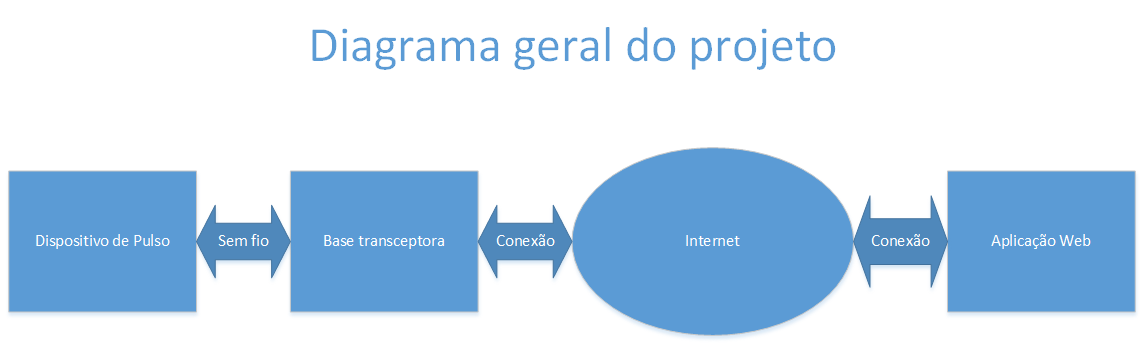
\includegraphics[scale=0.75]{figuras/diagrama_geral}
\end{center}

\subsubsection{Diagrama do dispositivo de pulso}
\begin{center}
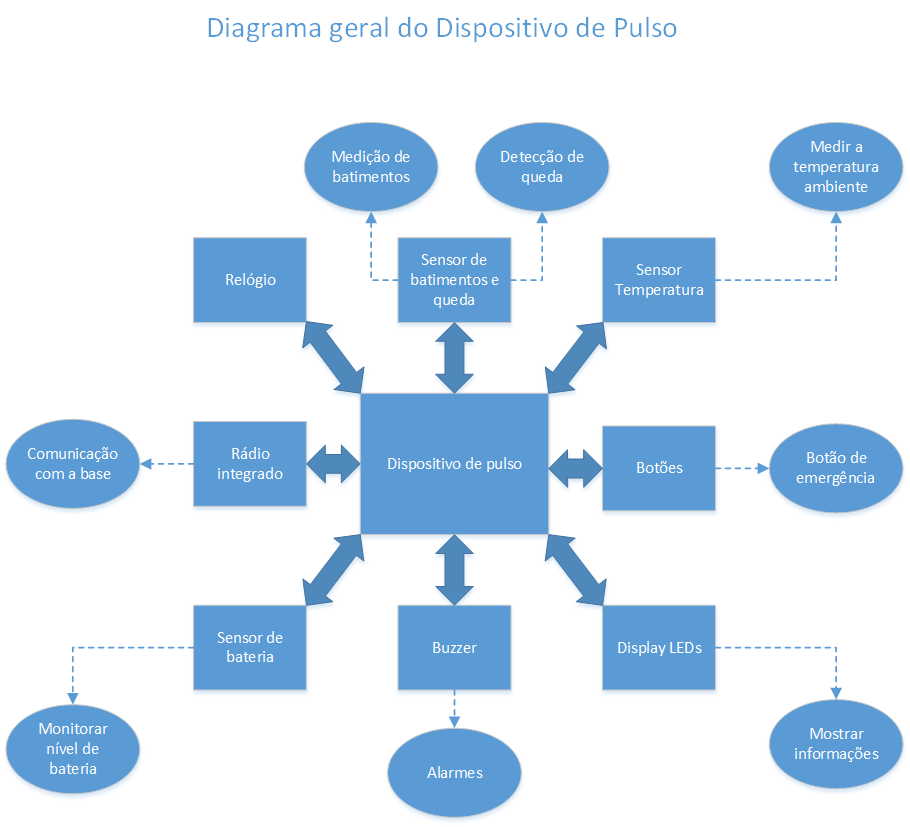
\includegraphics[scale=0.75]{figuras/diagrama_pulso}
\end{center}

\subsubsection{Diagrama da base transreceptora}
\begin{center}
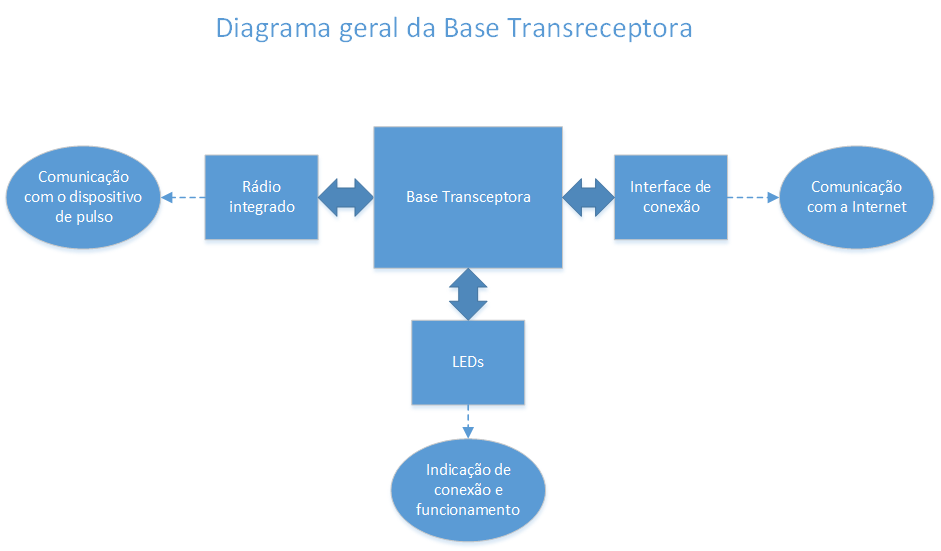
\includegraphics[scale=0.75]{figuras/diagrama_base}
\end{center}

\subsubsection{Diagrama da aplicação web}
\begin{center}
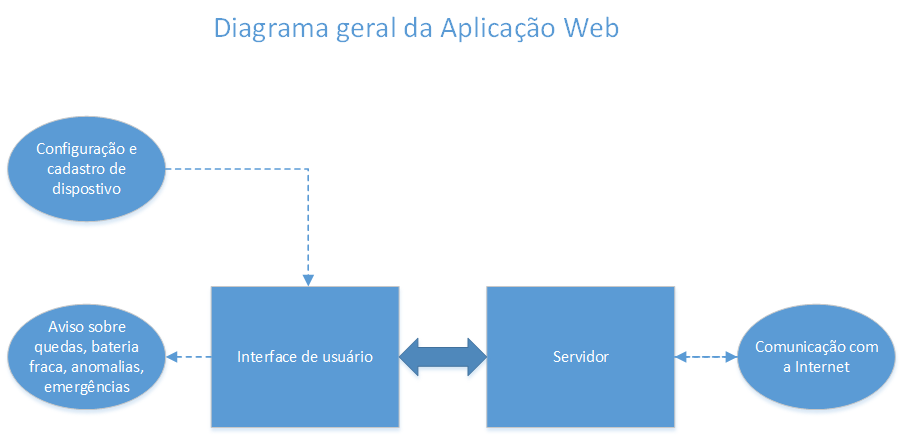
\includegraphics[scale=0.75]{figuras/diagrama_web}
\end{center}

\section{JUSTIFICATIVA E RESULTADOS ESPERADOS}

\subsection{Justificativa Resumida}
A população idosa vem crescendo de forma consistente durante décadas, devido ao aumento da qualidade e expectativa de vida \cite{KUCHEMANN2012}. Esta parte da população requer atenção e cuidados especiais, devidos aos problemas de saúde típicos da idade avançada, um terço dos atendimentos à lesões traumáticas são para pessoas com mais de 60 anos \cite{CALERTA}. A tecnologia atual permite que seja feito um monitoramento remoto e não invasivo do idoso, porém o mercado carece de produtos que venham a promover a tranquilidade tanto para os familiares quanto para os médicos que cuidam dessas pessoas. Com as mudanças socioeconômicas entre 1992 e 2012 ocorreu um aumento de 235\% no número de idosos que vivem sozinhos \cite{FOLHA} e é em casa onde 75\% dos acidentes com idosos acontecem \cite{ACRIT}.

Por monitorar condições de saúde, detectar quedas e possuir um botão de emergência para o idoso, este pode viver mais livre e tranquilo, sabendo que está sendo cuidado de forma remota e que, caso qualquer coisa aconteça, o serviço médico urgente será alertado. O rápido atendimento é essência para diminuição de riscos à vida do paciente e para o aumento de suas chances de recuperação, em caso de infarto - por exemplo - o antedimento deve ocorrer dentro de no máximo 90 minutos \cite{CALERTA}.


\subsection{Resultados Esperados}
Com o desenvolvimento desse projeto visa-se oferecer um prototipo funcional de um produto que pode ser amadurecido para chegar ao mercado, se houver aceitação e investimentos. 

\subsubsection{Tecnológicos}
\begin{itemize}
\item O protótipo de um sistema eletrônico de monitoramento para idosos.
\item Uma interface web compatível com o sistema desenvolvido.
\end{itemize}

\subsubsection{Científicos}
\begin{itemize}
\item Não aplicável.
\end{itemize}

\subsubsection{Econômicos}
\begin{itemize}
\item Protótipo de um produto que pode ser colocado no mercado.
\item Uma nova opção de monitoramento de idosos para famílias, planos de saúde, médicos etc.
\end{itemize}

\subsubsection{Sociais}
\begin{itemize}
\item O uso da tecnologia por parte da população para monitorar pessoas idosas.
\end{itemize}

\section{METODOLOGIA E MECANISMOS DE GESTÃO}

\subsection{Metodologia}
Para que o desenvolvimento do projeto seja consistente, as seguintes etapas e seus devidos resultados esperados são mostrados a seguir.

\subsubsection{}
\begin{itemize}
\item Estudo dos requisitos de software, como IDE, paradigma de programação, e hardware, como alimentação e interfaces, necessários para o projeto: com isso pode-se iniciar o desenvolvimento tanto do software quanto do hardware.
\item Definição dos protocolos de comunicação entre as três partes do projeto: visa manter o desenvolvimento desacoplado e garantir coerência nas etapas de integração.
\item Desenvolvimento das partes independentemente: ter as três partes do projeto prontas, ainda a serem testadas, tanto software como hardware.
\subitem Dispositivo de pulso: pesquisa para a aquisição dos batimentos cardíacos, algoritmo para detectar quedas, desenvolvimento do firmware;
\subitem Base transceptora: levantamento do hardware necessário, desenvolvimento do firmware;
\subitem Aplicação Web: levantamento de requisitos do servidor, desenvolvimento das requisições;
\item Testes individuais: ter cada parte do projeto testada individualmente, para garantir que não existam erros graves dentro de cada parte.
\item Testes de Integração: ter o sistema testado com todas as partes integradas, garantindo o seu funcionamento.
\end{itemize}

\subsection{Cronograma Resumido e Datas Importantes}
Início do Projeto: 29/02/2016. \\

Desenvolvimento da proposta: 29/02/2016 a 01/06/2016. 

Apresentação da proposta: 01/06/2016 a 01/07/2016. \\

Pesquisas preliminares: 01/07/2016 a 12/07/2016.

Desenvolvimento do dispostivo de pulso: 12/07/2016 a 29/11/2016.

Desenvolvimento da base transceptora: 12/07/2016 a 27/09/2016.

Desenvolvimento da Aplicação web: 12/07/2016 a 30/08/2016. \\

Testes de integração: 29/11/2016 a 03/01/2017.

Testes de validação: 03/01/2017 a 24/01/2017. \\

Escrita de Monografia: 01/06/16 a 04/04/2017.

Preparação da apresentação: 04/04/2017 a 18/04/2017. \\

Apresentação: 18/04/2017 a 30/06/2017.

\subsection{Cronograma Detalhado}
\begin{center}
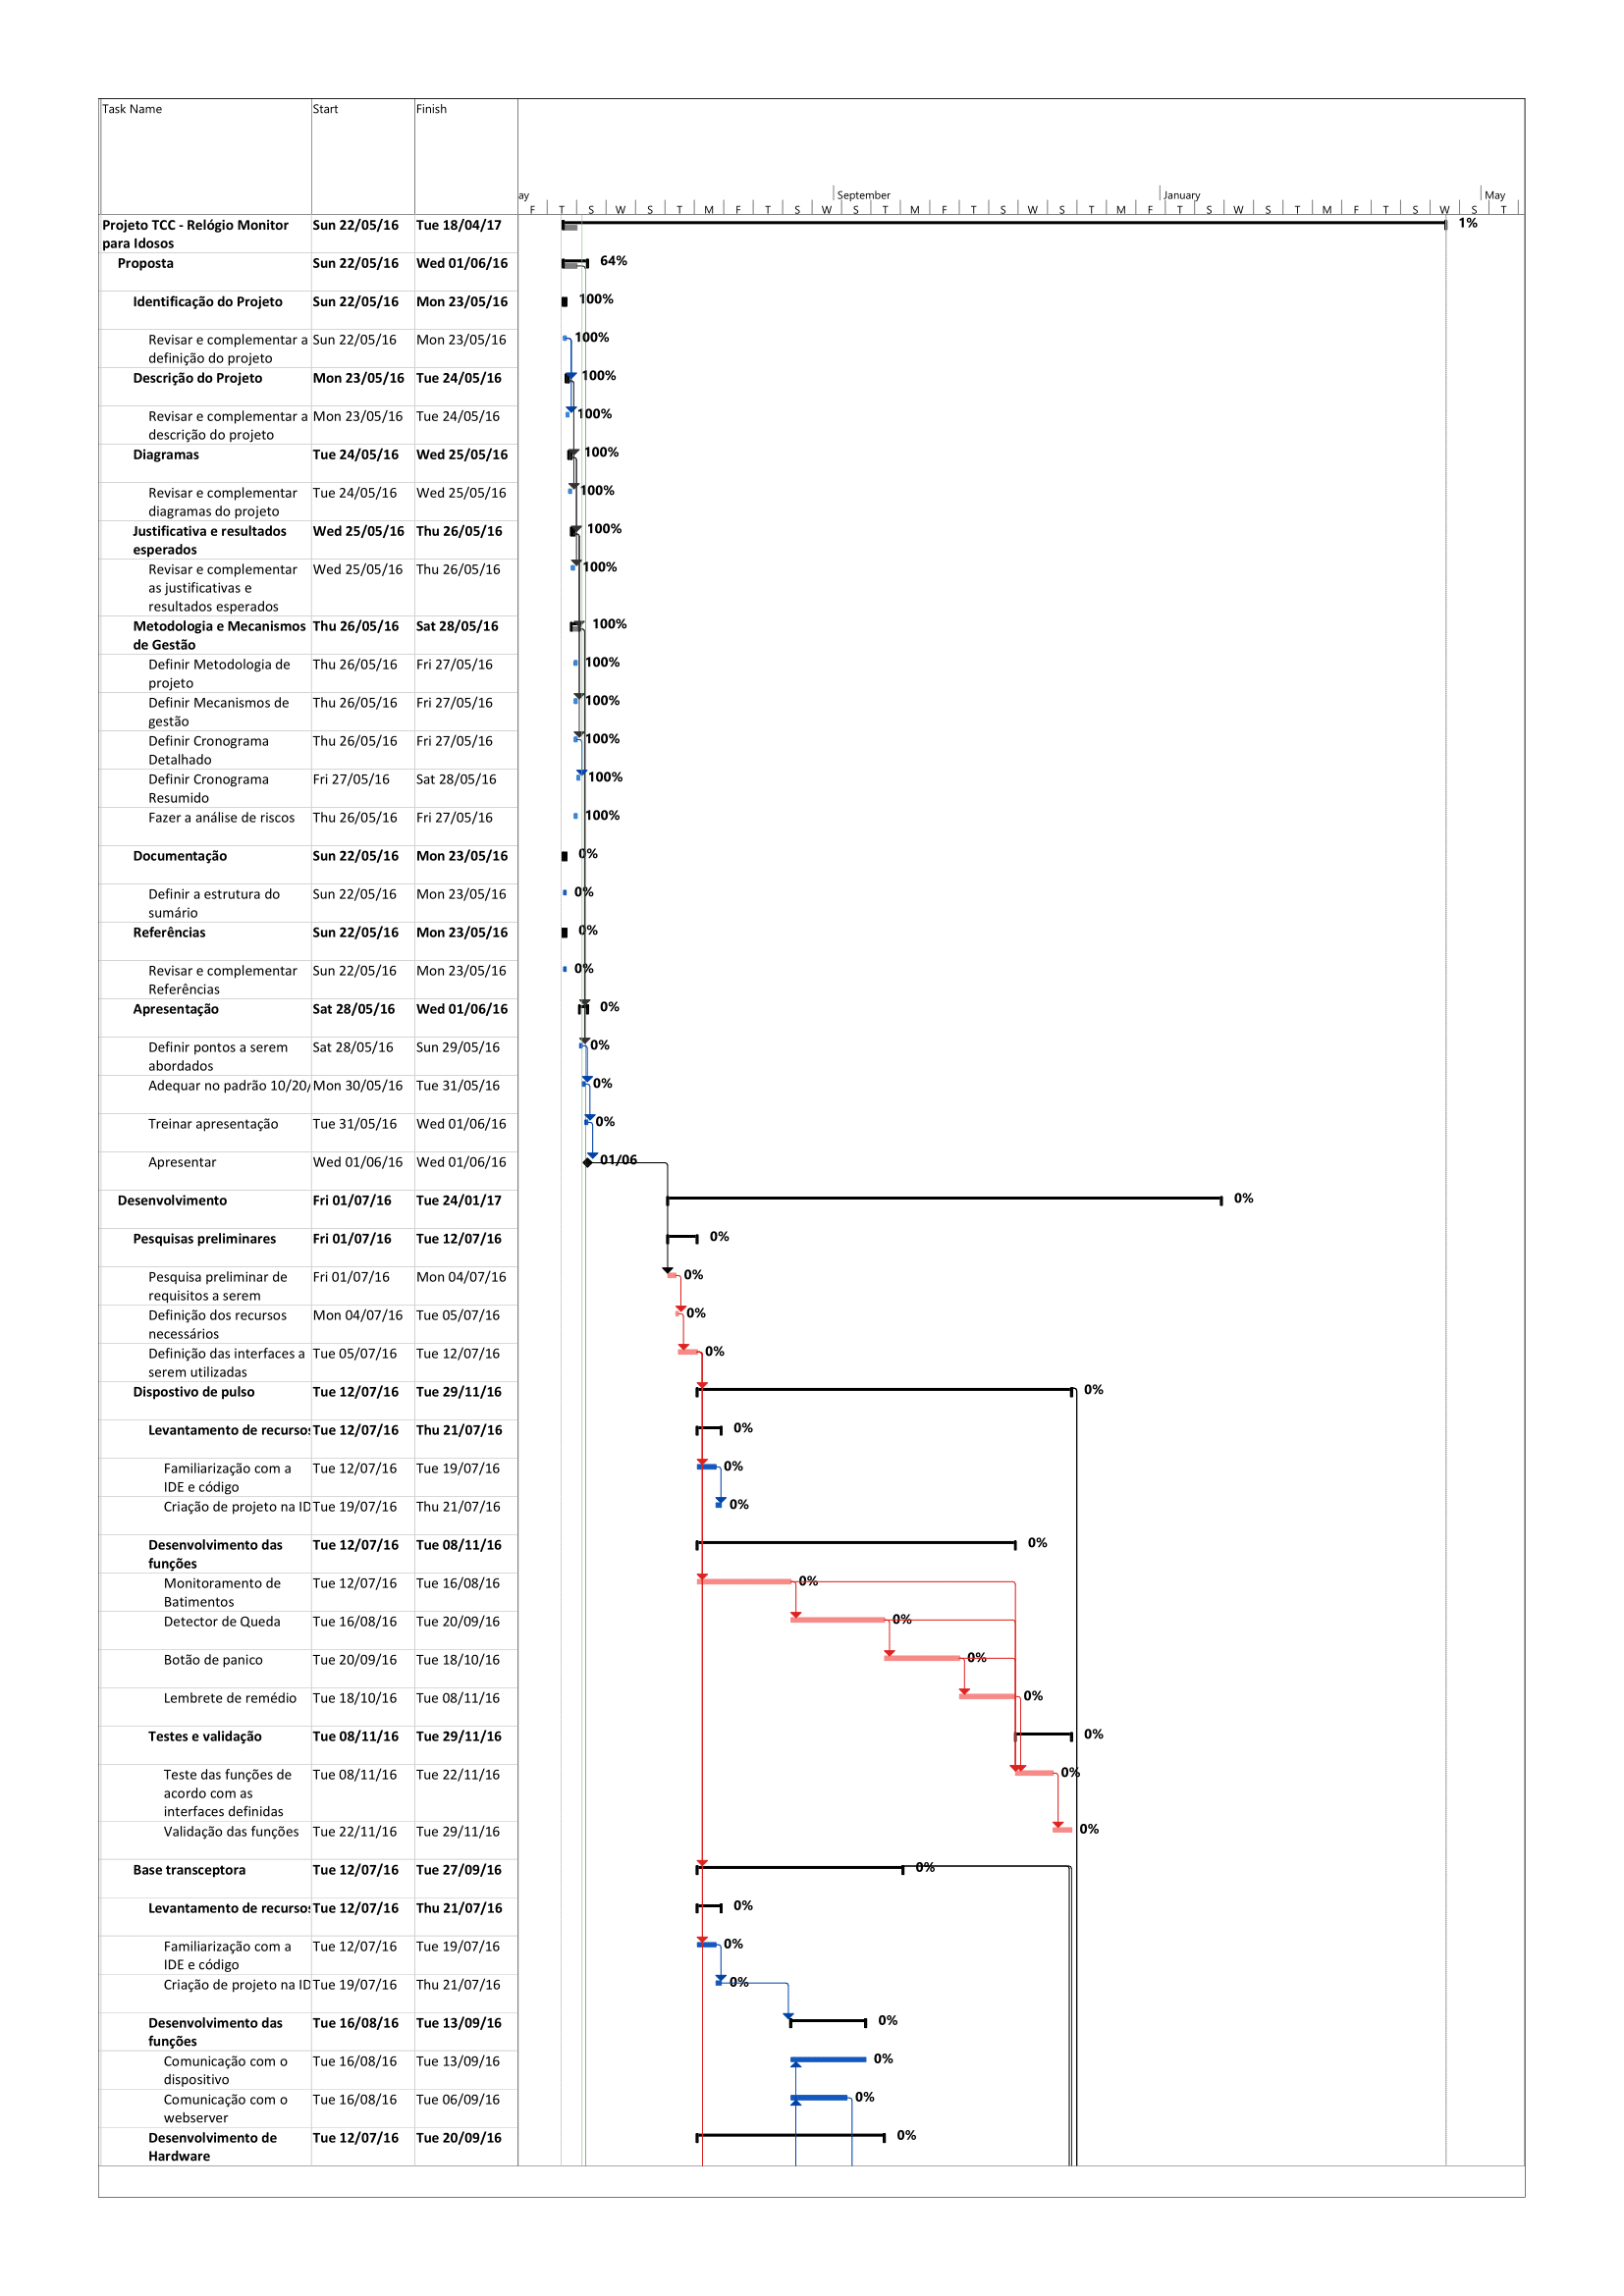
\includegraphics[scale=0.29]{figuras/Cronograma-1.png}
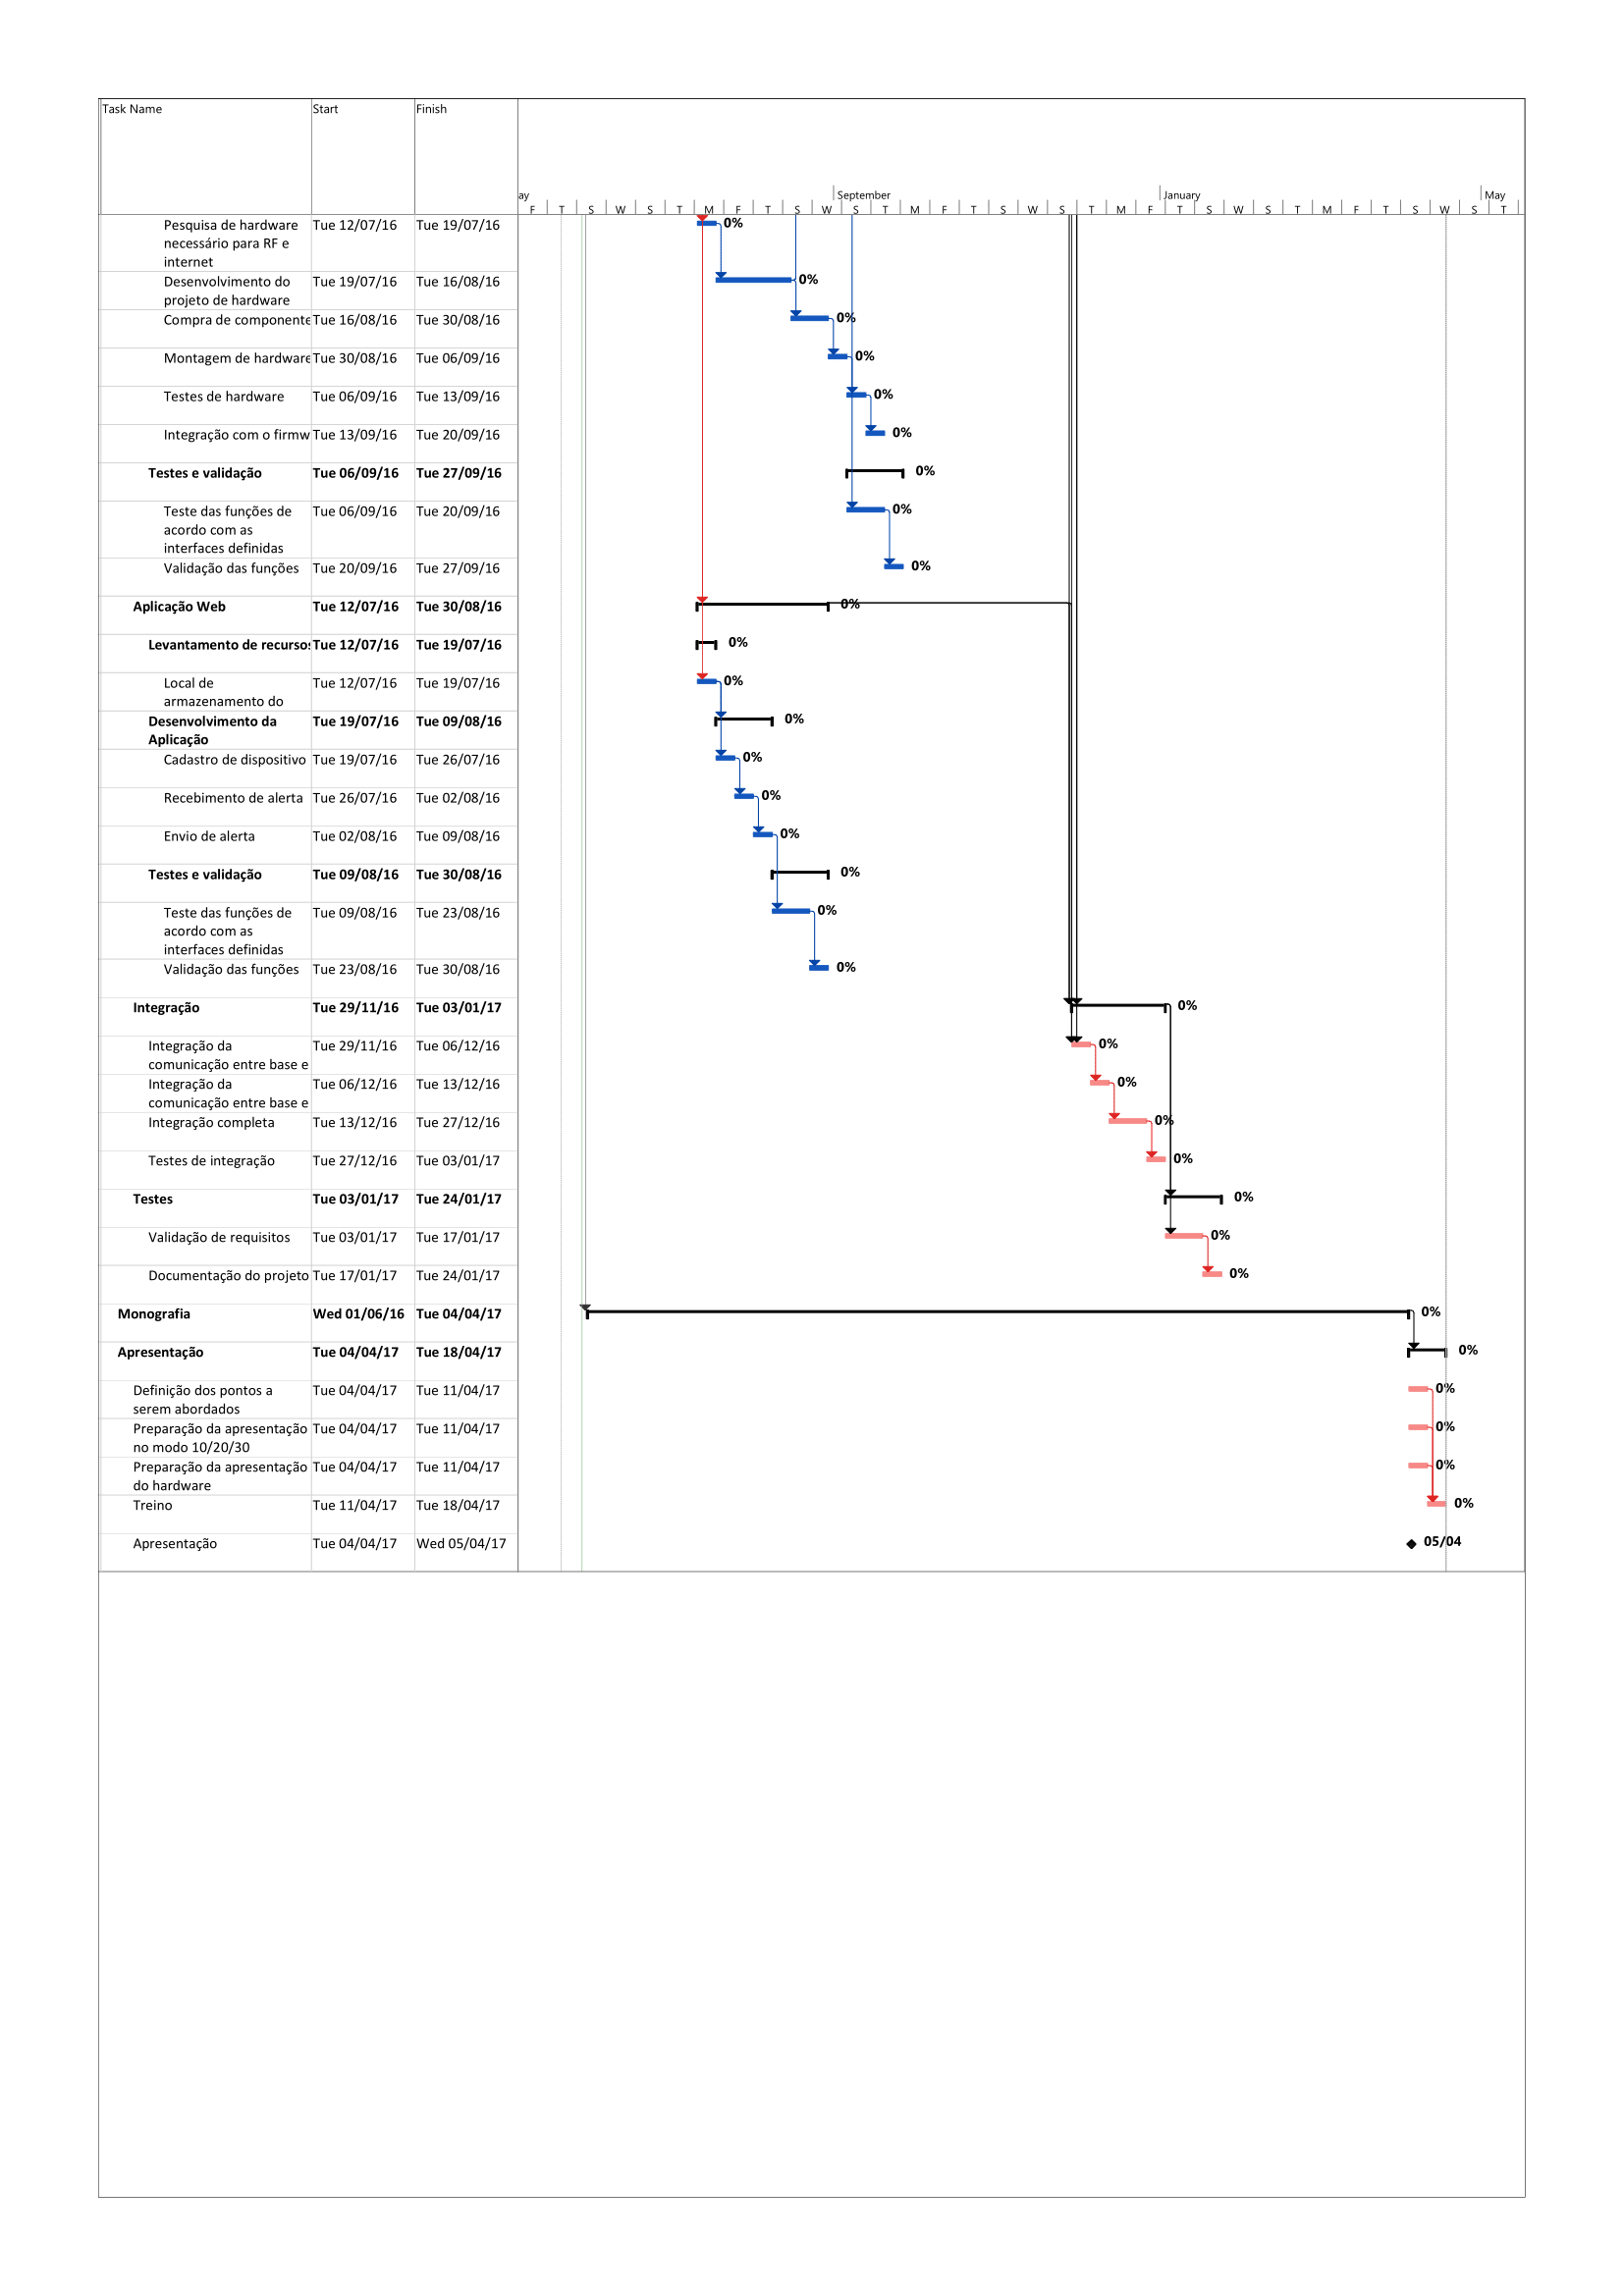
\includegraphics[scale=0.29]{figuras/Cronograma-2.png}
\end{center}
\subsection{Análise de Riscos}
Como todo projeto de engenharia, existem riscos que devem ser considerados no desenvolvimento, sendo os principais mostrados a seguir.

\subsubsection{Aquisição de batimentos cardíacos errática}
Devido à exposição do dispotivo à situações cotidianas impossíveis de serem previstas, é possível que existam situações em que o dispositivo venha a adquirir os batimentos cardíacos de maneira errada, causado por vibrações, movimentos, etc. Senso assim, é necessário que haja um algoritmo para detectar se a medição dos batimentos é confiável ou não. Como este fator possui BAIXO RISCO de acontecer, mas como causa um impacto direto na confiabilidade do sistema, é classificado como ALTO IMPACTO.
\subsubsection{Não detecção de quedas}
Pelo mesmo motivo de não ser possível prever todas as situações pelas quais o dispotivo irá passar, podem ocorrer situações em que quedas são indevidamente identificadas ou não identificadas. Assim, vários testes devem serem feitos para que a detecção das quedas seja ampla. Este fator atua diretamente sobre a confiabilidade do sistema, tendo BAIXO RISCO e ALTO IMPACTO.
\subsubsection{Duração da bateria}
Por ser um dispositivo portátil, é importante que o mesmo tenha uma bateria de longa duração. O projeto visa atingir um nível de consumo de forma a bateria ser trocada apenas em intervalos de pelo menos 3 meses. Se por algum motivo o consumo seja maior que o esperado, o produto terá um atrativo menor, porém sem perder a sua função principal. Por isso, classifica-se como BAIXO RISCO e possui BAIXO IMPACTO.
\subsubsection{Alcance reduzido}
Por utilizar de radiofrequencia para a comunicação com a base, existe a possibilidade que o alcance do dispositivo não seja suficiente para cobrir uma casa por completo, por exemplo. Isso causaria um impacto na utilização do sistema, pois limitaria o espaço em que o sistema funcionaria de forma completa. Apesar de não impedir o funcionamento, irá o limitar e pode causar consequencias mais sérias. Portanto classifica-se como MÉDIO RISCO e MÉDIO IMPACTO.
\subsubsection{Comunicação com a internet}
A única forma de o dispotivo se comunicar com o mundo externo é através da internet, sendo assim é de extrema importância que a comunicação tenha altos indíces de funcionamento. Por ser baixa a possibilidade de não existir comunicação com a internet, classifica-se como BAIXO RISCO, porém como é uma função vital para o projeto, classifica-se como ALTO IMPACTO.
\subsubsection{Aceitação pelo mercado e usuários}
Apesar de ser ainda um protótipo, é interessante que o mercado venha a aceitar a ideia, e portanto possibilitando o desenvolvimento de um produto final. Por não ser o objetivo do projeto, especificamente, um produto final, classifica-se como BAIXO RISCO e BAIXO IMPACTO.

\section{DOCUMENTAÇÃO}

\subsection{Estrutura do sumário}

\begin{enumerate}[label*=\arabic*.]

  	\item INTRODUÇÃO
    
    \item MOTIVAÇÃO
    
    \item DEFINIÇÃO DO PROBLEMA

	\item OBJETIVO
	
  	\item GESTÃO
	\begin{enumerate}[label*=\arabic*.]
		\item Escopo
		\item Cronograma
		\item Custos
		\item Riscos
		\item Considerações
	\end{enumerate} 
    
    \item REQUISITOS

	\item DESENVOLVIMENTO
	\begin{enumerate}[label*=\arabic*.]
		\item Dispostivo de pulso
		\begin{enumerate}[label*=\arabic*.]
			\item Hardware
			\item Firmware
		\end{enumerate}
		\item Base transceptora
		\begin{enumerate}[label*=\arabic*.]
			\item Hardware
			\item Firmware
		\end{enumerate}
		\item Aplicação Web
		\begin{enumerate}[label*=\arabic*.]
			\item Servidor
			\item Requisições
		\end{enumerate}
	\end{enumerate}

	\item TESTES
    
    \item VALIDAÇÀO DO SISTEMA
    
	\item PLANO DE NEGÓCIOS
	
	\item DISCUSSÃO
    
    \item CONCLUSÃO
    
    \item REFERÊNCIAS
    	

\end{enumerate}

\bibliographystyle{plain}
\nocite {KUCHEMANN2012,CALERTA,ACRIT,FOLHA}

\bibliography{refs}

\end{document}